\documentclass[12pt,titlepage,a4page , tikz , multi,table , svgnames,xcdraw]{article}
\usepackage{graphicx}
\usepackage[svgnames , table , xcdraw]{xcolor} 
\usepackage{fancyhdr}
 
\usepackage{hyperref}
\hypersetup{
    colorlinks=true,
    linkcolor=blue,
    filecolor=magenta,      
    urlcolor=cyan,
}

\usepackage{mathtools}
\usepackage{multirow}
\usepackage{graphicx}
\usepackage{float}
\usepackage{enumitem}
\usepackage{listings }
\usepackage[a4paper, total={6in, 8in}]{geometry}
\usepackage{afterpage}
\usepackage{amssymb}
\usepackage{pdflscape}
\usepackage{lscape}
\usepackage{amsmath}
\usepackage{svg}
\usepackage[final]{pdfpages}

\usepackage{pgf, tikz}
\usetikzlibrary{arrows, automata}
\usetikzlibrary{shapes.multipart}


\usepackage[T1]{fontenc}
\usepackage{tikz}
\usepackage[utf8]{inputenc} % Required for inputting international characters
\usepackage{PTSerif} 

\usepackage{float}

\usepackage[Kashida]{xepersian}
\settextfont[
 BoldFont={XB NiloofarBd.ttf}
 ]{XB Niloofar.ttf}


\NewDocumentCommand{\codeword}{v}{
\texttt{\textcolor{blue}{#1}}
}
\DeclareFixedFont{\ttb}{T1}{txtt}{bx}{n}{12} % for bold
\DeclareFixedFont{\ttm}{T1}{txtt}{m}{n}{12}  % for normal


\definecolor{deepblue}{rgb}{0,0,0.5}
\definecolor{deepred}{rgb}{0.6,0,0}
\definecolor{deepgreen}{rgb}{0,0.5,0}
\definecolor{mGreen}{rgb}{0,0.6,0}
\definecolor{mGray}{rgb}{0.5,0.5,0.5}
\definecolor{mPurple}{rgb}{0.58,0,0.82}
\definecolor{backgroundColour}{rgb}{0.95,0.95,0.95}


\newcommand\independent{\protect\mathpalette{\protect\independenT}{\perp}}
\def\independenT#1#2{\mathrel{\rlap{$#1#2$}\mkern2mu{#1#2}}}

% Python style for highlighting
\newcommand\pythonstyle{\lstset{
language=Python,
basicstyle=\ttm,
otherkeywords={self},             % Add keywords here
keywordstyle=\ttb\color{deepblue},
emph={MyClass,__init__},          % Custom highlighting
emphstyle=\ttb\color{deepred},    % Custom highlighting style
stringstyle=\color{deepgreen},
frame=tb,                         % Any extra options here
showstringspaces=false            % 
}}

\lstdefinestyle{CStyle}{
    backgroundcolor=\color{backgroundColour},   
    commentstyle=\color{mGreen},
    keywordstyle=\color{magenta},
    numberstyle=\tiny\color{mGray},
    stringstyle=\color{mPurple},
    basicstyle=\footnotesize,
    breakatwhitespace=false,         
    breaklines=true,                                   
    keepspaces=true,                 
    numbers=left,                    
    numbersep=5pt,                  
    showspaces=false,                
    showstringspaces=false,
    showtabs=false,                  
    tabsize=2,
    language=C,
}

\lstset{emph={%  
    uint64_t
    },emphstyle={\color{mGreen}}%
}%

\lstdefinelanguage
   [test]{Assembler}     % add a "x64" dialect of Assembler
    % based on the "x86masm" dialect
   % with these extra keywords:
   {morekeywords={rightrotate, xor , and , not , xor }} % etc.

\lstset{language=[test]Assembler}

% Python environment
\lstnewenvironment{python}[1][]
{
\pythonstyle
\lstset{#1}
}
{}

% Python for external files
\newcommand\pythonexternal[2][]{{
\pythonstyle
\lstinputlisting[#1]{#2}}}

\newenvironment{changemargin}[2]{%
\begin{list}{}{%
\setlength{\topsep}{0pt}%
\setlength{\leftmargin}{#1}%
\setlength{\rightmargin}{#2}%
\setlength{\listparindent}{\parindent}%
\setlength{\itemindent}{\parindent}%
\setlength{\parsep}{\parskip}%
}%
\item[]}{\end{list}}

% Python for inline
\newcommand\pythoninline[1]{{\pythonstyle\lstinline!#1!}}


\begin{document}

\begin{titlepage}

 \begin{center}
        
       \vspace*{1cm}

 \vspace{1cm}
       \textbf{ \Huge{به نام خدا} }
       \vspace{0.4cm}
       
       
\includegraphics[width=0.4\textwidth]{sharif.png}
       
 	\vspace{0.7cm}
       \textbf{ \LARGE{معماری کامپیوتر} }

 
   \vspace{0.7cm}
  \textbf{ \Large{ پروژهٔ پایانی - بخش دوم - شبیه‌سازی \lr{gem5}} }
   \vspace{0.5cm}
       
 
      \large \textbf{دانشکدهٔ مهندسی کامپیوتر}\\\vspace{0.2cm}
    \large   دانشگاه صنعتی شریف\\\vspace{0.25cm}
      
استاد:\\
    \textbf{{جناب آقای دکتر اسدی}}

    \vspace{0.15cm}
    \noindent\rule[1ex]{\linewidth}{3pt}
    
    \vspace{0.5cm}
نام، نام خانوادگی و شمارهٔ دانشجویی اعضای گروه:\\
    \textbf{{سپهر پورقناد - 97101359}}
        \vspace{0.1cm}
        
     \textbf{{سیدمحمدصادق کشاورزی - 97106249}}
        \vspace{0.1cm}
        
       \textbf{{امیرمهدی نامجو - 97107212}}
        \vspace{0.1cm}


\end{center}
\end{titlepage}

\newpage
\pagestyle{fancy}
\fancyhf{}
\fancyfoot{}

\cfoot{\thepage}
\chead{پروژهٔ پایانی}
\rhead{شبیه‌ساز \lr{gem5}}
\lhead{معماری کامپیوتر}

\newpage
\section{بررسی دستورات}
الگوریتم
\lr{SHA-256}
دارای دو دسته از دستورات است که به صورت دستورات رایج
\lr{ISA}
نیست. در واقع این دستورات ترکیبی از چند دستور رایج
\lr{ISA}
هستند که مقادیر محاسبه‌شدهٔ میانی دوباره استفاده نمی‌شوند. اگر هر کدام از این دستورات را بتوان در مدت زمان یک دستور رایج
\lr{ISA}
انجام داد، سرعت اجرای برنامه سریع‌تر می‌شود. این دو دسته به صورت زیر هستند:


دسته اول:

\begin{latin}
\begin{lstlisting}[columns=flexible]
s0 := (w[i-15] rightrotate  7) xor (w[i-15] rightrotate 18)
 xor (w[i-15] rightshift 3)
 
s1 := (w[i- 2] rightrotate 17) xor (w[i- 2] rightrotate 19)
 xor (w[i- 2] rightshift 10)
 
w[i] := w[i-16] + s0 + w[i-7] + s1
\end{lstlisting}
\end{latin}
\par
\par
دسته دوم:

\begin{latin}
\begin{lstlisting}[columns=flexible]
S1 := (e rightrotate 6) xor (e rightrotate 11) xor (e rightrotate 25)
ch := (e and f) xor ((not e) and g)
temp1 := h + S1 + ch + k[i] + w[i]
S0 := (a rightrotate 2) xor (a rightrotate 13) xor (a rightrotate 22)
maj := (a and b) xor (a and c) xor (b and c)
\end{lstlisting}
\end{latin}


هر کدام از دستورات بالا گزینه‌ای برای اضافه کردن به
\lr{ISA}
است.

 ما در اینجا دستور
\lr{\texttt{a = (b \& c) \^ (\textasciitilde b \& d)}}
پیاده‌سازی می‌کنیم و اثر آن بر بهبود سرعت اجرای برنامه را بررسی می‌کنیم.
\newpage
\section{اضافه کردن دستور}
فایل
\lr{\texttt{src/arch/x86/isa/decoder/two\_byte\_opcodes.isa}}:

\begin{latin}
\begin{verbatim}
0x56: mynewop({{
    Rax = PseudoInst::mynewop(xc->tcBase(), Rdi, Rsi, Rdx);
}}, IsNonSpeculative);
\end{verbatim}
\end{latin}


\par
فایل
\lr{\texttt{src/sim/pseudo\_inst.cc}}:
\begin{latin}
\begin{lstlisting}[style=CStyle]
uint64_t
mynewop(ThreadContext *tc, uint64_t arg1, uint64_t arg2, uint64_t arg3)
{
    quiesceCycle(tc, 100);
    return (((arg1) & (arg2)) ^ (~(arg1) & (arg3)));
}
\end{lstlisting}
\end{latin}


\par
که تأخیر اجرای دستور را (بر حسب تعداد چرخهٔ ساعت) به عنوان ورودی به دستور
\lr{\texttt{quiesceCycle}}
می‌دهیم (که در مثال بالا برابر ۱۰۰ چرخهٔ ساعت است).
\par
۳ تأخیر زیر را برای این دستور در نظر می‌گیریم:
\begin{enumerate}
\item
۱ چرخهٔ ساعت: که حالت ایده‌آل است.
\item
۲۰ چرخهٔ ساعت: که برابر تعداد چرخهٔ لازم برای اجرای این دستور در پردازندهٔ
\lr{multicycle}
آموزش‌داده‌شده در درس است (با فرض موجود بودن متغیرها در ثبات‌ها).
\item
۱۰۰ چرخهٔ ساعت: که تخمینی برای حد بالای تعداد چرخهٔ لازم برای اجرای این دستور در پردازندهٔ ۸۰۸۶ است (با فرض موجود بودن متغیرها در حافظه).
\end{enumerate}
زمان‌های اجرا به ازای رشتهٔ ورودی
\lr{"how are you doing today?"}
 به شرح زیر است:
\begin{enumerate}
\item
\lr{ISA}
اصلی: ۱۶۳٬۰۲۱٬۰۰۰ تیک
\item
دستور اختصاصی با تأخیر ۱ چرخهٔ ساعت: ۱۶۳٬۴۶۰٬۰۰۰ تیک
$\leftarrow$
بهبود = ۰٫۹۹۷ (احتمالاً علت این که نه تنها بهبود نداشته‌ایم، بلکه زمان اجرا بدتر نیز شده‌است، این است که کامپایلر این دستور را نمی‌شناسد و اجرای این دستور جدید، بهینه‌سازی‌های کامپایلر (از جمله تخصیص ثبات) را به هم می‌ریزد و از بین می‌برد).
\item
دستور اختصاصی با تأخیر ۲۰ چرخهٔ ساعت: ۱۶۴٬۰۶۸٬۰۰۰ تیک
$\leftarrow$
بهبود = ۰٫۹۹۳
\item
دستور اختصاصی با تأخیر ۱۰۰ چرخهٔ ساعت: ۳۲٬۱۶۳٬۴۲۸٬۰۰۰ تیک
$\leftarrow$
بهبود = ۰٫۰۰۵۰۶
\end{enumerate}
همهٔ حالات با تنظیمات
\lr{\texttt{se.py}}
بدون هیچ تغییری اجرا شدند و هر ثانیه برابر
$10^{12}$
تیک است.
\newpage
\section{تأثیر حافظه نهان}
\begin{itemize}
\item
\lr{ISA}
اصلی:
\begin{itemize}
\item
بدون حافظهٔ نهان: ۱۳٬۲۸۸٬۷۳۰٬۰۰۰ تیک
\item
حافظهٔ نهان دوسطحی: ۷۳۵٬۴۷۴٬۰۰۰ تیک
$\leftarrow$
بهبود = ۱۸٫۰۶۸
\end{itemize}
تعداد دسترسی‌های خواندن‌ داده از حافظه از ۴۵۰۵۲ به ۴۵۰۴۶ و نوشتن دستور به حافظه از ۱۹۹۸۴۳ به ۱۹۹۷۵۶ کاهش یافته‌است. تعداد دسترسی‌ها و
\lr{miss}های
دیگر تغییر نداشته‌است.
\item
دستور اختصاصی با تأخیر ۱۰۰ چرخهٔ ساعت:
\begin{itemize}
\item
بدون حافظهٔ نهان: ۱۳٬۳۳۲٬۸۹۴٬۰۰۰
\item
حافظهٔ نهان دوسطحی: ۷۴۲٬۸۴۳٬۰۰۰
$\leftarrow$
بهبود = ۱۷٫۹۴۸
\end{itemize}
تعداد خواندن‌های داده از حافظه نیز از ۴۵۰۵۲ به ۴۵۰۴۶ و تعداد نوشتن‌های دستور به حافظه از ۲۰۰۶۳۴ به ۲۰۰۵۴۷ کاهش یافته‌است. تعداد دسترسی‌ها و
\lr{miss}های
دیگر تغییر نداشته‌است.
\end{itemize}
\newpage
\section{تنظیمات حافظه نهان}
اثر پارامترهای مختلف بر کارایی برنامه را در حالت استفاده از دستور اختصاصی با تأخیر ۱۰۰ چرخهٔ ساعت بررسی می‌کنیم:
\begin{itemize}
\item
بدون تغییرات: ۷۴۲٬۸۴۳٬۰۰۰ تیک (در این حالت
\lr{associativity}
برابر ۶۴ است.)
\item
\lr{Cacheline}:
\begin{itemize}
\item
۳۲: ۸۷۳٬۷۷۹٬۰۰۰
$\leftarrow$
بهبود = ۰٫۸۵۰
\item
۶۴: ۷۸۲٬۸۴۳٬۰۰۰؛
احتمالاً مقدار از پیش تعیین‌شدهٔ این پارامتر در سیستم همین مقدار است و به همین علت هیچ بهبودی مشاهده نمی‌شود.
\end{itemize}
\item
\lr{L2 Cache Associativity}:
\begin{itemize}
\item
۸: ۷۴۲٬۸۴۳٬۰۰۰
\item
۱۶: ۷۴۲٬۸۴۳٬۰۰۰
\end{itemize}
در واقع در اجراهای مختلف مشاهده شد که زمان اجرا به ازای مقادیر مختلف این پارامتر به غیر از ۱ با یکدیگر برابر هستند، که احتمالاً به علت کم بودن تعداد برخوردها در حافظهٔ نهان است. به طور کلی تقریباً همهٔ آمار و ارقام مربوط به دو مقدار متفاوت
\lr{associativity}
با یکدیگر برابر بودند که احتمالاً به دلیل تعداد کم متغیرهای موجود در برنامه، و تکرار عملیات یکسان در طی اجرا است.
\end{itemize}

\newpage
\section{ساختار اتصالات پیاده‌سازی شده در فایل‌های تنظیمات}
ساختار کلی سیستم (اتصالات بین کش‌ها و مموری و پردازنده) که در فایل‌های اصلی تنظیمات ارسالی پیاده سازی شده به صورت زیر است:

\begin{center}
\begin{latin}
\tikzset{every picture/.style={line width=0.75pt}} %set default line width to 0.75pt        

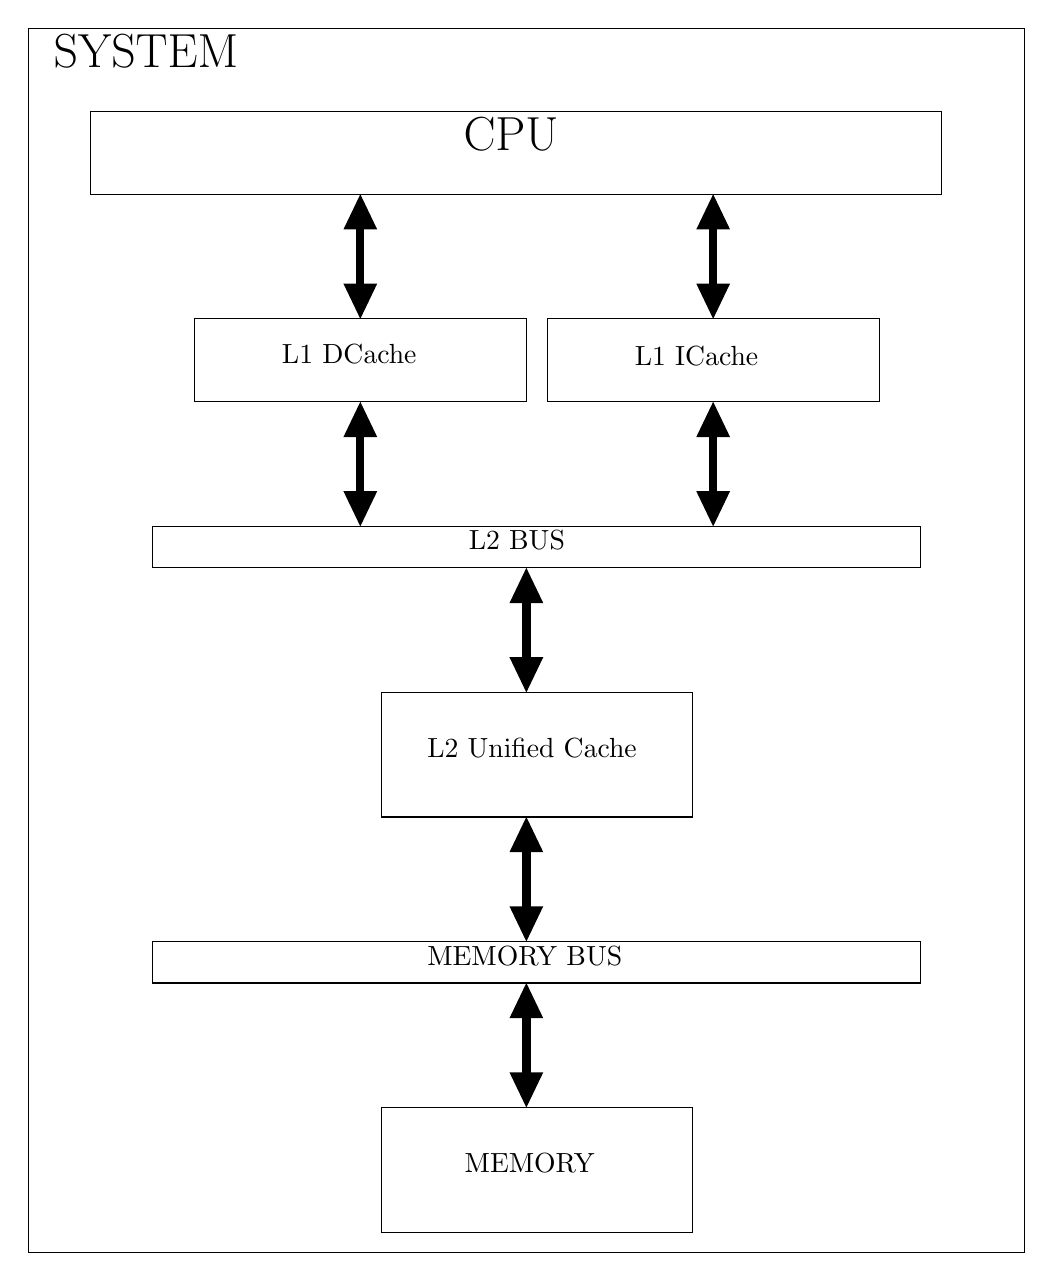
\begin{tikzpicture}[x=0.75pt,y=0.75pt,yscale=-1,xscale=1]
%uncomment if require: \path (0,684); %set diagram left start at 0, and has height of 684

%Shape: Rectangle [id:dp36610427966804293] 
\draw   (110,100) -- (520,100) -- (520,140) -- (110,140) -- cycle ;
%Shape: Rectangle [id:dp8044312760122254] 
\draw   (160,200) -- (320,200) -- (320,240) -- (160,240) -- cycle ;
%Shape: Rectangle [id:dp21011322278976174] 
\draw   (330,200) -- (490,200) -- (490,240) -- (330,240) -- cycle ;
%Shape: Rectangle [id:dp509234216391141] 
\draw   (140,300) -- (510,300) -- (510,320) -- (140,320) -- cycle ;
%Shape: Rectangle [id:dp9094728166203774] 
\draw   (250,380) -- (400,380) -- (400,440) -- (250,440) -- cycle ;
%Shape: Rectangle [id:dp6825872712664733] 
\draw   (140,500) -- (510,500) -- (510,520) -- (140,520) -- cycle ;
%Shape: Rectangle [id:dp06128240971614307] 
\draw   (250,580) -- (400,580) -- (400,640) -- (250,640) -- cycle ;
%Shape: Rectangle [id:dp725424768485041] 
\draw   (80,60) -- (560,60) -- (560,650) -- (80,650) -- cycle ;
%Straight Lines [id:da5610493858704471] 
\draw [line width=3]    (240,146) -- (240,194) ;
\draw [shift={(240,200)}, rotate = 270] [fill={rgb, 255:red, 0; green, 0; blue, 0 }  ][line width=0.08]  [draw opacity=0] (16.97,-8.15) -- (0,0) -- (16.97,8.15) -- cycle    ;
\draw [shift={(240,140)}, rotate = 90] [fill={rgb, 255:red, 0; green, 0; blue, 0 }  ][line width=0.08]  [draw opacity=0] (16.97,-8.15) -- (0,0) -- (16.97,8.15) -- cycle    ;
%Straight Lines [id:da9800774482945052] 
\draw [line width=3]    (410,146) -- (410,194) ;
\draw [shift={(410,200)}, rotate = 270] [fill={rgb, 255:red, 0; green, 0; blue, 0 }  ][line width=0.08]  [draw opacity=0] (16.97,-8.15) -- (0,0) -- (16.97,8.15) -- cycle    ;
\draw [shift={(410,140)}, rotate = 90] [fill={rgb, 255:red, 0; green, 0; blue, 0 }  ][line width=0.08]  [draw opacity=0] (16.97,-8.15) -- (0,0) -- (16.97,8.15) -- cycle    ;
%Straight Lines [id:da6539257254568029] 
\draw [line width=3]    (410,246) -- (410,294) ;
\draw [shift={(410,300)}, rotate = 270] [fill={rgb, 255:red, 0; green, 0; blue, 0 }  ][line width=0.08]  [draw opacity=0] (16.97,-8.15) -- (0,0) -- (16.97,8.15) -- cycle    ;
\draw [shift={(410,240)}, rotate = 90] [fill={rgb, 255:red, 0; green, 0; blue, 0 }  ][line width=0.08]  [draw opacity=0] (16.97,-8.15) -- (0,0) -- (16.97,8.15) -- cycle    ;
%Straight Lines [id:da8196206823592931] 
\draw [line width=3]    (240,246) -- (240,294) ;
\draw [shift={(240,300)}, rotate = 270] [fill={rgb, 255:red, 0; green, 0; blue, 0 }  ][line width=0.08]  [draw opacity=0] (16.97,-8.15) -- (0,0) -- (16.97,8.15) -- cycle    ;
\draw [shift={(240,240)}, rotate = 90] [fill={rgb, 255:red, 0; green, 0; blue, 0 }  ][line width=0.08]  [draw opacity=0] (16.97,-8.15) -- (0,0) -- (16.97,8.15) -- cycle    ;
%Straight Lines [id:da299556369694824] 
\draw [line width=3]    (320,326) -- (320,374) ;
\draw [shift={(320,380)}, rotate = 270] [fill={rgb, 255:red, 0; green, 0; blue, 0 }  ][line width=0.08]  [draw opacity=0] (16.97,-8.15) -- (0,0) -- (16.97,8.15) -- cycle    ;
\draw [shift={(320,320)}, rotate = 90] [fill={rgb, 255:red, 0; green, 0; blue, 0 }  ][line width=0.08]  [draw opacity=0] (16.97,-8.15) -- (0,0) -- (16.97,8.15) -- cycle    ;
%Straight Lines [id:da22073201667516784] 
\draw [line width=3]    (320,446) -- (320,494) ;
\draw [shift={(320,500)}, rotate = 270] [fill={rgb, 255:red, 0; green, 0; blue, 0 }  ][line width=0.08]  [draw opacity=0] (16.97,-8.15) -- (0,0) -- (16.97,8.15) -- cycle    ;
\draw [shift={(320,440)}, rotate = 90] [fill={rgb, 255:red, 0; green, 0; blue, 0 }  ][line width=0.08]  [draw opacity=0] (16.97,-8.15) -- (0,0) -- (16.97,8.15) -- cycle    ;
%Straight Lines [id:da23592429489394862] 
\draw [line width=3]    (320,526) -- (320,574) ;
\draw [shift={(320,580)}, rotate = 270] [fill={rgb, 255:red, 0; green, 0; blue, 0 }  ][line width=0.08]  [draw opacity=0] (16.97,-8.15) -- (0,0) -- (16.97,8.15) -- cycle    ;
\draw [shift={(320,520)}, rotate = 90] [fill={rgb, 255:red, 0; green, 0; blue, 0 }  ][line width=0.08]  [draw opacity=0] (16.97,-8.15) -- (0,0) -- (16.97,8.15) -- cycle    ;

% Text Node
\draw (281,102) node [anchor=north west][inner sep=0.75pt]   [align=left] {\begin{minipage}[lt]{39.959656pt}\setlength\topsep{0pt}
\begin{flushright}
{\LARGE CPU}
\end{flushright}

\end{minipage}};
% Text Node
\draw (201,211) node [anchor=north west][inner sep=0.75pt]   [align=left] {L1 DCache};
% Text Node
\draw (371,212) node [anchor=north west][inner sep=0.75pt]   [align=left] {L1 ICache};
% Text Node
\draw (291,301) node [anchor=north west][inner sep=0.75pt]   [align=left] {L2 BUS};
% Text Node
\draw (271,401) node [anchor=north west][inner sep=0.75pt]   [align=left] {L2 Unified Cache};
% Text Node
\draw (271,501) node [anchor=north west][inner sep=0.75pt]   [align=left] {MEMORY BUS};
% Text Node
\draw (289,601) node [anchor=north west][inner sep=0.75pt]   [align=left] {MEMORY};
% Text Node
\draw (91,62) node [anchor=north west][inner sep=0.75pt]   [align=left] {{\LARGE SYSTEM}};


\end{tikzpicture}
\end{latin}
\end{center}

\newpage
\section{فایل‌های تحویل داده شده}
در پوشه مربوط به این پروژه،‌ چند فایل و یک پوشه به نام Stats قرار دارد. فایل \lr{sha256.cpp} کد به زبان \lr{C++} الگوریتم \lr{SHA256} است که در بخش main آن،‌ این الگوریتم روی رشته 
\lr{"how are you doing today?"}
اجرا شده است.

دو فایل \lr{caches.py} و \lr{main\_config.py} مربوط به حالت توصیف شده در سوال هستند و در فایل cahces تنظیمات مربوط به cache ها قرار گرفته است و در فایل \lr{main\_config.py} تنظیمات کلی مربوط به سایر قطعات و در نهایت اتصالات آن‌ها قرار دارد. یک فایل دیگر هم به نام \lr{withoutcache.py} وجود دارد که مربوط به تنظیمات بدون استفاده از حافظه نهان است.


درون پوشه \lr{Stats} سه پوشه با نام‌های \lr{Phase1} و \lr{Phase2} و \lr{Phase3} قرار دارد. \lr{Phase1} مربوط به نتایج اجرای برنامه در اثر اضافه کردن دستور با سه تاخیر (۱ و ۲۰ و ۱۰۰ چرخه ساعت) گفته شده در صفحات قبل است. \lr{Phase2} مربوط به نتیجه اجرا با و بدون استفاده از کش است. \lr{Phase3} مربوط به تست کردن حالات مختلف \lr{cacheline} و \lr{associativity} که در مستند پروژه گفته شده بود است. درون هر کدام از پوشه‌ها، فایل‌های \lr{.txt} خروجی‌های \lr{GEM5} قرار گرفته است.
\end{document}












